

\tikzset{every picture/.style={line width=0.75pt}} %set default line width to 0.75pt        

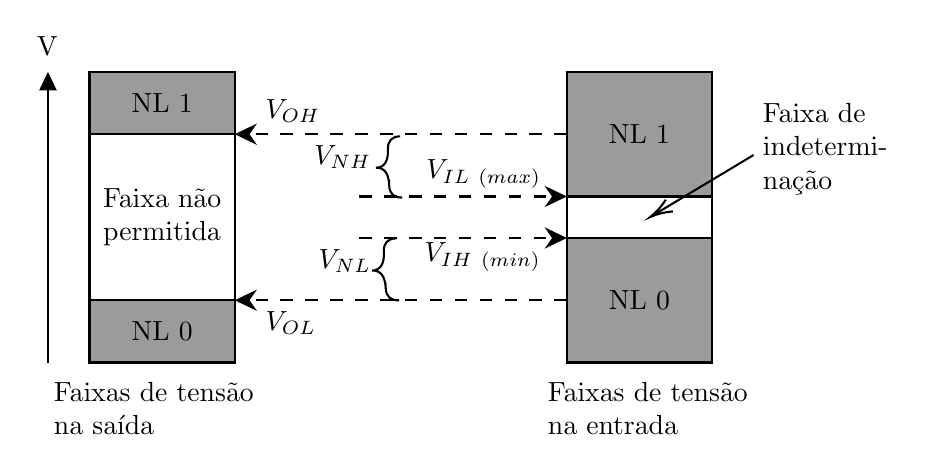
\begin{tikzpicture}[x=0.75pt,y=0.75pt,yscale=-1,xscale=1]
%uncomment if require: \path (0,300); %set diagram left start at 0, and has height of 300

%Straight Lines [id:da9362711052123074] 
\draw    (30,170) -- (30,32) ;
\draw [shift={(30,30)}, rotate = 450] [fill={rgb, 255:red, 0; green, 0; blue, 0 }  ][line width=0.75]  [draw opacity=0] (8.93,-4.29) -- (0,0) -- (8.93,4.29) -- cycle    ;

%Shape: Rectangle [id:dp4032147941400168] 
\draw  [fill={rgb, 255:red, 155; green, 155; blue, 155 }  ,fill opacity=1 ] (50,140) -- (120,140) -- (120,170) -- (50,170) -- cycle ;
%Shape: Rectangle [id:dp7848825407478928] 
\draw  [fill={rgb, 255:red, 155; green, 155; blue, 155 }  ,fill opacity=1 ] (50,30) -- (120,30) -- (120,60) -- (50,60) -- cycle ;
%Shape: Rectangle [id:dp39210423941486794] 
\draw   (50,60) -- (120,60) -- (120,140) -- (50,140) -- cycle ;
%Shape: Rectangle [id:dp11801813712916065] 
\draw  [fill={rgb, 255:red, 155; green, 155; blue, 155 }  ,fill opacity=1 ] (280,30) -- (350,30) -- (350,90) -- (280,90) -- cycle ;
%Shape: Rectangle [id:dp4244461507786699] 
\draw  [fill={rgb, 255:red, 155; green, 155; blue, 155 }  ,fill opacity=1 ] (280,110) -- (350,110) -- (350,170) -- (280,170) -- cycle ;
%Shape: Rectangle [id:dp8601874700592713] 
\draw   (280,90) -- (350,90) -- (350,110) -- (280,110) -- cycle ;
%Straight Lines [id:da3672163587892687] 
\draw  [dash pattern={on 4.5pt off 4.5pt}]  (280,60) -- (122,60) ;
\draw [shift={(120,60)}, rotate = 360] [fill={rgb, 255:red, 0; green, 0; blue, 0 }  ][line width=0.75]  [draw opacity=0] (10.72,-5.15) -- (0,0) -- (10.72,5.15) -- (7.12,0) -- cycle    ;

%Straight Lines [id:da8564463887662099] 
\draw  [dash pattern={on 4.5pt off 4.5pt}]  (180,90) -- (278,90) ;
\draw [shift={(280,90)}, rotate = 180] [fill={rgb, 255:red, 0; green, 0; blue, 0 }  ][line width=0.75]  [draw opacity=0] (10.72,-5.15) -- (0,0) -- (10.72,5.15) -- (7.12,0) -- cycle    ;

%Straight Lines [id:da37036161891510355] 
\draw  [dash pattern={on 4.5pt off 4.5pt}]  (180,110) -- (278,110) ;
\draw [shift={(280,110)}, rotate = 180] [fill={rgb, 255:red, 0; green, 0; blue, 0 }  ][line width=0.75]  [draw opacity=0] (10.72,-5.15) -- (0,0) -- (10.72,5.15) -- (7.12,0) -- cycle    ;

%Straight Lines [id:da35287999565207784] 
\draw  [dash pattern={on 4.5pt off 4.5pt}]  (280,140) -- (122,140) ;
\draw [shift={(120,140)}, rotate = 360] [fill={rgb, 255:red, 0; green, 0; blue, 0 }  ][line width=0.75]  [draw opacity=0] (10.72,-5.15) -- (0,0) -- (10.72,5.15) -- (7.12,0) -- cycle    ;

%Shape: Brace [id:dp8108628093433541] 
\draw   (199.68,61) .. controls (195.63,61.14) and (193.67,63.23) .. (193.81,67.28) -- (193.81,67.28) .. controls (194,73.07) and (192.08,76.03) .. (188.03,76.16) .. controls (192.08,76.03) and (194.2,78.85) .. (194.4,84.63)(194.31,82.03) -- (194.4,84.63) .. controls (194.53,88.68) and (196.63,90.64) .. (200.68,90.5) ;
%Shape: Brace [id:dp6109119495195752] 
\draw   (197.67,110.17) .. controls (193.57,110.38) and (191.63,112.53) .. (191.84,116.62) -- (191.84,116.62) .. controls (192.13,122.47) and (190.23,125.5) .. (186.14,125.71) .. controls (190.23,125.5) and (192.43,128.32) .. (192.72,134.17)(192.59,131.54) -- (192.72,134.17) .. controls (192.93,138.26) and (195.09,140.21) .. (199.18,140) ;
%Straight Lines [id:da7825021648757069] 
\draw    (370,70) -- (321.71,98.97) ;
\draw [shift={(320,100)}, rotate = 329.03999999999996] [color={rgb, 255:red, 0; green, 0; blue, 0 }  ][line width=0.75]    (10.93,-3.29) .. controls (6.95,-1.4) and (3.31,-0.3) .. (0,0) .. controls (3.31,0.3) and (6.95,1.4) .. (10.93,3.29)   ;


% Text Node
\draw (29.67,17.67) node  [align=left] {V};
% Text Node
\draw (85,45) node  [align=left] {NL 1};
% Text Node
\draw (85,155) node  [align=left] {NL 0};
% Text Node
\draw (85,100) node  [align=left] {Faixa não\\permitida};
% Text Node
\draw (315,60) node  [align=left] {NL 1};
% Text Node
\draw (315,140) node  [align=left] {NL 0};
% Text Node
\draw (148,49) node   {$V_{OH}$};
% Text Node
\draw (147,151) node   {$V_{OL}$};
% Text Node
\draw (240,79) node   {$V_{IL\ ( \text{max})}$};
% Text Node
\draw (239.5,119) node   {$V_{IH\ ( \text{min})}$};
% Text Node
\draw (172,71) node   {$V_{NH}$};
% Text Node
\draw (173,121) node   {$V_{NL}$};
% Text Node
\draw (404.5,67) node  [align=left] {Faixa de\\indetermi-\\nação};
% Text Node
\draw (81,192) node  [align=left] {Faixas de tensão\\na saída};
% Text Node
\draw (319,192) node  [align=left] {Faixas de tensão\\na entrada};


\end{tikzpicture}